\documentclass{beamer}

\usepackage[utf8]{inputenc}
\usepackage{forest}
\usepackage{tikz}
\usepackage{amsmath}
\usetikzlibrary{arrows,automata,positioning,backgrounds}
\usepackage[thicklines]{cancel}
\renewcommand{\CancelColor}{\color{red}}

\usetheme{default}
\beamertemplatenavigationsymbolsempty

\title{Ungleichungen von Kraft \& McMillan}
\subtitle{Proseminar Informationstheorie}
\author{Phil Pützstück}
\date{\today}

\newcommand{\up}[2]{\mathrel{\overset{\makebox[0pt]{\mbox{\normalfont\tiny #2}}}{#1}}}

\forestset{%
  only/.code args={<#1>}{%
    \alt<#1>{}{\pgfkeysalso{before typesetting nodes={remove}}}
  },
}

\begin{document}
\maketitle

\begin{frame}
    \frametitle{Motivation}
    \begin{itemize}
        \setlength\itemsep{2em}
        \item Gesehen, dass eindeutig bzw. sofort dekodierbare Codes sehr nützlich sind.
        \item Wann bzw. unter welchen Bedingungen existieren diese?
        \item Insbesondere: Wortlängen und Größe des Code-Alphabets
        \item Vorgestellte Ungleichungen geben untere Schranken für diese
    \end{itemize}
\end{frame}

\begin{frame}
    \frametitle{Überblick}
    \begin{itemize}
        \setlength\itemsep{2em}
        \item Zusammenhang Codes und Bäume
        \item Ungleichung von Kraft
        \item Ungleichung von McMillan
        \item Bemerkungen / Zusammenfassung
    \end{itemize}
\end{frame}

\begin{frame}[t]
    \frametitle{Code als Baum: $\mathcal{T}_r^h$}
    Höhe $h \in \mathbb{N}$, Verzweigungsgrad $r \in \mathbb{N}$.
    \\Beispiel $r=3,h=2$, Baum $\mathcal{T}_3^2$:
    \begin{center}
        \only<1>{
        \Large
        \begin{forest}
            [$v_\varepsilon$
                [$v_0$
                    [$v_{00}$],
                    [$v_{01}$],
                    [$v_{02}$]
                ],
                [$v_1$
                    [$v_{10}$],
                    [$v_{11}$],
                    [$v_{12}$]
                ],
                [$v_2$
                    [$v_{20}$],
                    [$v_{21}$],
                    [$v_{22}$]
                ]
            ]
        \end{forest}\\
        }
        \only<2>{
        \Large
        \begin{forest}
            [$v_\varepsilon$
                [$v_0$,alias=d,edge={line width =1pt}, edge label = {node[midway,above,sloped,alias=e]{1}}
                    [$v_{00}$, edge={line width =1pt}, edge label = {node[red,midway, above, sloped]{2}}],
                    [$v_{01}$],
                    [$v_{02}$]
                ],
                [$v_1$
                    [$v_{10}$],
                    [$v_{11}$],
                    [$v_{12}$]
                ],
                [$v_2$,
                    [$v_{20}$],
                    [$v_{21}$],
                    [$v_{22}$]
                ]
            ]
            \node at (-3.85,0) {\small$|00| = {\color{red}2}$};
            \draw[<->] (-5.3,-2.5) to[bend left] (-4.5,-0.1);
        \end{forest}\\
        }

        \only<3->{
        \Large
        \begin{forest}
            [$v_{\color{red}\varepsilon}$
                [$v_0$
                    [$v_{00}$],
                    [$v_{01}$],
                    [$v_{02}$]
                ],
                [$v_{\color{red}1}$, edge label={node [midway, sloped, above] {\color{blue}$\leq$}}
                    [$v_{{\color{red}1}0}$, edge label={node [midway, sloped, above] {\color{blue}$\geq$}}],
                    [$v_{{\color{red}1}1}$, edge label={node [midway, sloped, above] {\normalsize\color{blue}$\leq$}}],
                    [$v_{{\color{red}1}2}$, edge label={node [midway, sloped, above] {\color{blue}$\leq$}}]
                ],
                [$v_2$
                    [$v_{20}$],
                    [$v_{21}$],
                    [$v_{22}$]
                ]
            ],
        \end{forest}\\
        }
    \end{center}
    \pause
    \begin{itemize}
        \setlength\itemsep{2em}
        \item Knoten $v_w$ hat Höhe $|w|$
        \pause
        \item Für $v_w, v_{w'}$ gelte
            $v_w\ {\color{blue}\leq}\ v_{w'} \,\Longleftrightarrow\, w\ {\color{red}\sqsubseteq}\ w'$
    \end{itemize}
\end{frame}

\section{Ungleichung von Kraft}
\begin{frame}
    \frametitle{Ungleichung von Kraft}
    Seien $q,r \in \mathbb{N}, \ell \in \mathbb{N}^q$. Dann existiert ein $r$-ärer sofort dekodierbarer Code $\mathcal{C}$
    mit Wortlängen $\ell$ genau dann, wenn
    $$
        \sum_{k=1}^{q} \frac{1}{r^{\ell_k}} \leq 1
    $$\\[20pt]
    \pause

    Annahmen:

    \begin{itemize}
        \setlength\itemsep{1em}
        \item Anzahl Code-Wörter $q > 1$
        \item Wortlängen $0 < \ell_1 \leq \ell_2 \leq \cdots \leq \ell_q$
            aufsteigend sortiert
        \item Code-Alphabet von $\mathcal{C}$ ist $[0,r-1]$
    \end{itemize}
\end{frame}

\begin{frame}[t]
    \frametitle{Ungleichung von Kraft: Beweisidee ''$\,\Longrightarrow\,$''}
    Bekannt: $\mathcal{C}$ sofort dekodierbar $\,\Longleftrightarrow\,$ $\mathcal{C}$ Präfixcode.\\[5pt]
    Beispiel:
    $
    q=3,
    {\only<2>{\color{red}}r=2},
    \ell=(
    {\only<3>{\color{blue}}1},
    {\only<7>{\color{blue}}2},
    {\only<2,11>{\color{blue}}3})
    $.
    \only<2-12>{
        Betrachte
        \only<2-5>{$\mathcal{T}_{\only<2>{\color{red}}2}^{\only<2>{\color{blue}}3}$}
        \only<6-9>{{\only<6>{\color{red}}$\mathcal{T}_2^3 \setminus v_0$}}
        \only<10-12>{{\only<10>{\color{red}}$(\mathcal{T}_2^3 \setminus v_0) \setminus v_{11}$}}
        \\
        \only<4-12>{
            {\only<4>{\color{blue}}$w_1 = {\only<5>{\color{red}}0}$},
            \only<8-12>{
                {\only<8>{\color{blue}}$w_2 = {\only<9>{\color{red}}11}$},
                \only<12>{{\color{blue}$w_3 = 101$}}
            }
        }
    }
    \strut\\[20pt]
    \onslide{
        \only<2>{
            \begin{center}
                \begin{forest}
                    [$v_\varepsilon$
                        [$v_0$
                            [$v_{00}$
                                [$v_{000}$],
                                [$v_{001}$]
                            ],
                            [$v_{01}$
                                [$v_{010}$],
                                [$v_{011}$]
                            ]
                        ],
                        [$v_1$
                            [$v_{10}$
                                [$v_{100}$],
                                [$v_{101}$]
                            ],
                            [$v_{11}$
                                [$v_{110}$],
                                [$v_{111}$]
                            ]
                        ]
                    ]
                \end{forest}
            \end{center}
        }
        \only<3>{
            \begin{center}
                \begin{forest}
                    [$v_\varepsilon$
                        [$v_0$,blue,draw
                            [$v_{00}$
                                [$v_{000}$],
                                [$v_{001}$]
                            ],
                            [$v_{01}$
                                [$v_{010}$],
                                [$v_{011}$]
                            ]
                        ],
                        [$v_1$,blue,draw
                            [$v_{10}$
                                [$v_{100}$],
                                [$v_{101}$]
                            ],
                            [$v_{11}$
                                [$v_{110}$],
                                [$v_{111}$]
                            ]
                        ]
                    ]
                \end{forest}
            \end{center}
        }
        \only<4>{
            \begin{center}
                \begin{forest}
                    [$v_\varepsilon$
                        [$v_0$,draw,blue
                            [$v_{00}$
                                [$v_{000}$],
                                [$v_{001}$]
                            ],
                            [$v_{01}$
                                [$v_{010}$],
                                [$v_{011}$]
                            ]
                        ],
                        [$v_1$
                            [$v_{10}$
                                [$v_{100}$],
                                [$v_{101}$]
                            ],
                            [$v_{11}$
                                [$v_{110}$],
                                [$v_{111}$]
                            ]
                        ]
                    ]
                \end{forest}
            \end{center}
        }
        \only<5>{
            \begin{center}
                \begin{forest}
                    [$v_\varepsilon$
                        [$v_{\color{red}0}$
                            [$v_{{\color{red}0}0}$
                                [$v_{{\color{red}0}00}$],
                                [$v_{{\color{red}0}01}$]
                            ],
                            [$v_{{\color{red}0}1}$
                                [$v_{{\color{red}0}10}$],
                                [$v_{{\color{red}0}11}$]
                            ]
                        ],
                        [$v_1$
                            [$v_{10}$
                                [$v_{100}$],
                                [$v_{101}$]
                            ],
                            [$v_{11}$
                                [$v_{110}$],
                                [$v_{111}$]
                            ]
                        ]
                    ]
                \end{forest}
            \end{center}
        }
        \only<6>{
            \begin{center}
                \begin{forest}
                    [$v_\varepsilon$
                        [$v_0$,red,edge={dashed},
                            [$v_{00}$,red
                                [$v_{000}$,red],
                                [$v_{001}$,red]
                            ],
                            [$v_{01}$,red
                                [$v_{010}$,red],
                                [$v_{011}$,red]
                            ]
                        ],
                        [$v_1$
                            [$v_{10}$,
                                [$v_{100}$],
                                [$v_{101}$]
                            ],
                            [$v_{11}$,
                                [$v_{110}$],
                                [$v_{111}$]
                            ]
                        ]
                    ]
                \end{forest}
            \end{center}
        }
        \only<7>{
            \begin{center}
                \begin{forest}
                    [$v_\varepsilon$
                        [$v_0$,red,edge={dashed},
                            [$v_{00}$,red,draw,dashed
                                [$v_{000}$,red],
                                [$v_{001}$,red]
                            ],
                            [$v_{01}$,red,draw,dashed
                                [$v_{010}$,red],
                                [$v_{011}$,red]
                            ]
                        ],
                        [$v_1$
                            [$v_{10}$,draw,blue
                                [$v_{100}$],
                                [$v_{101}$]
                            ],
                            [$v_{11}$,draw,blue
                                [$v_{110}$],
                                [$v_{111}$]
                            ]
                        ]
                    ]
                \end{forest}
            \end{center}
        }
        \only<8>{
            \begin{center}
                \begin{forest}
                    [$v_\varepsilon$
                        [$v_0$,red,edge={dashed},
                            [$v_{00}$,red
                                [$v_{000}$,red],
                                [$v_{001}$,red]
                            ],
                            [$v_{01}$,red
                                [$v_{010}$,red],
                                [$v_{011}$,red]
                            ]
                        ],
                        [$v_1$
                            [$v_{10}$,
                                [$v_{100}$],
                                [$v_{101}$]
                            ],
                            [$v_{11}$,draw,blue
                                [$v_{110}$],
                                [$v_{111}$]
                            ]
                        ]
                    ]
                \end{forest}
            \end{center}
        }
        \only<9>{
            \begin{center}
                \begin{forest}
                    [$v_\varepsilon$
                        [$v_0$,red,edge={dashed}
                            [$v_{00}$,red
                                [$v_{000}$,red],
                                [$v_{001}$,red]
                            ],
                            [$v_{01}$,red
                                [$v_{010}$,red],
                                [$v_{011}$,red]
                            ]
                        ],
                        [$v_1$
                            [$v_{10}$
                                [$v_{100}$],
                                [$v_{101}$]
                            ],
                            [$v_{\color{red}11}$
                                [$v_{{\color{red}11}0}$],
                                [$v_{{\color{red}11}1}$]
                            ]
                        ]
                    ]
                \end{forest}
            \end{center}
        }
        \only<10>{
            \begin{center}
                \begin{forest}
                    [$v_\varepsilon$
                        [$v_0$,red,edge={dashed}
                            [$v_{00}$,red
                                [$v_{000}$,red],
                                [$v_{001}$,red]
                            ],
                            [$v_{01}$,red
                                [$v_{010}$,red],
                                [$v_{011}$,red]
                            ]
                        ],
                        [$v_1$
                            [$v_{10}$
                                [$v_{100}$],
                                [$v_{101}$]
                            ],
                            [$v_{11}$,red,edge={dashed}
                                [$v_{110}$,red],
                                [$v_{111}$,red]
                            ]
                        ]
                    ]
                \end{forest}
            \end{center}
        }
        \only<11>{
            \begin{center}
                \begin{forest}
                    [$v_\varepsilon$
                        [$v_0$,red,edge={dashed}
                            [$v_{00}$,red
                                [$v_{000}$,red,draw,dashed],
                                [$v_{001}$,red,draw,dashed]
                            ],
                            [$v_{01}$,red
                                [$v_{010}$,red,draw,dashed],
                                [$v_{011}$,red,draw,dashed]
                            ]
                        ],
                        [$v_1$
                            [$v_{10}$
                                [$v_{100}$,draw,blue],
                                [$v_{101}$,draw,blue]
                            ],
                            [$v_{11}$,red,edge={dashed}
                                [$v_{110}$,red,draw,dashed],
                                [$v_{111}$,red,draw,dashed]
                            ]
                        ]
                    ]
                \end{forest}
            \end{center}
        }
        \only<12>{
            \begin{center}
                \begin{forest}
                    [$v_\varepsilon$
                        [$v_0$,red,edge={dashed}
                            [$v_{00}$,red
                                [$v_{000}$,red],
                                [$v_{001}$,red]
                            ],
                            [$v_{01}$,red
                                [$v_{010}$,red],
                                [$v_{011}$,red]
                            ]
                        ],
                        [$v_1$
                            [$v_{10}$
                                [$v_{100}$],
                                [$v_{101}$,draw,blue]
                            ],
                            [$v_{11}$,red,edge={dashed}
                                [$v_{110}$,red],
                                [$v_{111}$,red]
                            ]
                        ]
                    ]
                \end{forest}
            \end{center}
        }
    }
\end{frame}

\begin{frame}
    \frametitle{Ungleichung von Kraft: ''$\,\Longrightarrow\,$'': Induktionsanfang}
    \begin{columns}
    \begin{column}{0.7\textwidth}
        \visible<1->{
            \begin{itemize}
                \setlength\itemsep{1em}
                \item zz: Auswahl von $w_i$ aus Baum möglich.
                \item Via endlicher Induktion über $i$.
                \item $h := \ell_{max}$
            \end{itemize}\strut\\[20pt]\pause

            $i=1$:\\

            \begin{itemize}
                \setlength\itemsep{1em}
                \item Wähle Knoten ${\only<2>{\color{red}}v_w}$ der Höhe $\ell_1$
                \pause
                \item Setze $w_1 := w$, dann $|w_1| = \ell_1$
                \pause
                \item Entferne Nachfolger; $\mathcal{T}_1 := \mathcal{T}_r^h \setminus v_w$
            \end{itemize}
        }
    \end{column}

    \begin{column}{0.3\textwidth}
        \onslide
        \visible<2->{
            \quad$\mathcal{T}_r^h$:\\
            \begin{center}
                \begin{forest}
                    [$v_\varepsilon$
                        [$v_0$,
                            [\dots]
                        ],
                        [$v_1$
                            [\dots
                                [$v_w$,only=<2-3>,color=red,
                                    [$v_{w0}$
                                        [\dots]
                                    ],
                                    [$v_{w1}$
                                        [\dots]
                                    ],
                                    [\dots]
                                ],
                                [$v_w$,only=<4>,color=red,edge={dashed,red}
                                    [$v_{w0}$,red
                                        [\dots,red]
                                    ],
                                    [$v_{w1}$,red
                                        [\dots,red]
                                    ],
                                    [\dots,red]
                                ],
                            ],
                            [\dots]
                        ],
                        [\dots]
                    ]
                \end{forest}
            \end{center}
        }
    \end{column}
    \end{columns}
\end{frame}

\begin{frame}[t]
    \frametitle{Ungleichung von Kraft: ''$\,\Longrightarrow\,$'': Induktionsanfang}
    \begin{columns}
    \begin{column}{0.5\textwidth}
        \visible<1->{
            \begin{itemize}
                \setlength\itemsep{1em}
                \item Teilbaum der Höhe $h - \ell_1$ entfernt
                \pause
            \item $\mathcal{T}_1$ noch {\color{red}$r^h - r^{h-\ell_1}$} Blätter
            \end{itemize}\strut\\[10pt]\pause
        }
        Weiter gilt:
        \begin{overprint}
            \onslide<3>
            $$
                {\color{red}r^h - r^{h - \ell_1}}
                = r^h\bigg(1 - \sum_{k=1}^{1} \frac{1}{r^{\ell_k}}\bigg)
            $$
            \onslide<4>
            $$
                {\color{red}r^h - r^{h - \ell_1}}
                = r^h\bigg(1 - \sum_{k=1}^{1} \frac{1}{r^{\ell_k}}\bigg)
            $$
            $$
                {>}\ r^h\bigg(1 - \sum_{k=1}^{{\color{blue}q}} \frac{1}{r^{\ell_k}}\,\bigg )\visible<5>{> 0}
            $$
            \onslide<5>
            $$
                {\color{red}r^h - r^{h - \ell_1}}
                = r^h\bigg(1 - \sum_{k=1}^{1} \frac{1}{r^{\ell_k}}\bigg)
            $$
            $$
                {\color{red} >}\ r^h\bigg(1 - \underbrace{\sum_{k=1}^{q} \frac{1}{r^{\ell_k}}}_{\leq\ 1}\bigg)
                \geq {\color{red}0}
            $$
        \end{overprint}
    \end{column}

        \begin{column}{0.55\textwidth}
        \onslide
            \begin{center}
                \begin{tikzpicture}
                    \only<1>{\node[color=red] at (0.5,-3) {$v_{w_1}$};}
                    \only<2->{\node at (0.5,-3) {$v_{w_1}$};}
                    \node at (0,-1.5) {$\mathcal{T}_1$};

                    \draw (0,0) node[above]{$v_\varepsilon$}
                        -- (-2.5,-4)
                        -- (-.5,-4)
                        -- (0.5,-2.4)
                        -- (1.5,-4)
                        -- (2.5,-4)
                        -- cycle;

                    \draw[|-|] (3,-2.4) -- node[left] {$\ell_1$} (3, 0);
                    \draw[|-|] (3,-2.4) -- node[left] {\scriptsize{$h-\ell_1$}} (3, -4);
                    \draw[dotted, line width = .6pt] (3,-2.4) -- (0.5,-2.4);
                    \draw[dotted, line width = .6pt] (3,0) -- (0,0);
                    \draw[dotted, line width = .6pt] (2.5,-4) -- (3,-4);
                    \visible<2->{
                        \draw[|-|] (-.5,-4.5) -- node[below] {$r^{h-\ell_1}$} (1.5,-4.5);
                        \draw[|-|] (-2.5,-5.4) -- node[below] {$r^h$} (2.5,-5.4);
                        \draw[line width = 2pt,red] (-2.5,-4) -- (-.5,-4);
                        \draw[line width = 2pt,red] (1.5,-4) -- (2.5,-4);
                    }
                \end{tikzpicture}
            \end{center}
    \end{column}
    \end{columns}
\end{frame}

\begin{frame}[t]
    \frametitle{Ungleichung von Kraft: ''$\,\Longrightarrow\,$'': Induktionsschritt}

    \begin{columns}
    \begin{column}{0.7\textwidth}
        Induktionsvorraussetzungen für $i \in [1,q-1]$:
        \begin{itemize}
            \setlength\itemsep{.8em}
            \item $\forall j \in [1,i]: |w_j| = \ell_j$
            \item $\{w_j \mid j \in [1,i]\}$ Präfix-Code
            \item $\mathcal{T}_i$ mindestens 1 Blatt
        \end{itemize}\strut\\[10pt]
        \pause
        Dann:
        \begin{itemize}
            \setlength\itemsep{.8em}
            \pause
            \item Wähle {\color{red}$v_w$} der Höhe $\ell_{i+1} \leq h$
            \pause
            \item Setze $w_{i+1} := w$, da $|w_{i+1}| = \ell_{i+1}$
        \end{itemize}
    \end{column}
    \begin{column}{0.3\textwidth}\onslide
        \only<2->{
        \begin{center}
            \begin{tikzpicture}
                \node at (0,0) {$v_\varepsilon$};
                \node at (0,-4) {$v_x$};
                \visible<3->{\node[red] at (0,-2) {$v_w$};}

                \draw[dotted,line width = 1pt] (0,-0.5) -- (0,-1.5);
                \visible<2>{\draw[dotted,line width = 1pt] (0,-0.5) -- (0,-2.5);}
                \draw[dotted,line width = 1pt] (0,-2.5) -- (0,-3.5);

                \visible<3->{\draw[|-|] (.5, 0) -- node[right] {$\ell_{i+1}$}(.5, -2);}
                \draw[|-|] (1.5, 0) -- node[right] {$h$}(1.5, -4);
            \end{tikzpicture}
        \end{center}
        }
    \end{column}
    \end{columns}
\end{frame}

\begin{frame}[t]
    \frametitle{Ungleichung von Kraft: ''$\,\Longrightarrow\,$'': Induktionsschritt}
    Für $j \in [1,i]$:
    \begin{itemize}
        \setlength\itemsep{1em}
        \item Knoten ''unter'' $v_{w_j}$ bereits entfernt
        \pause
        \item Damit $v_{w_j} \not\leq v_{w_{i+1}}$, also auch $w_j \not\sqsubseteq w_{i+1}$
%        \pause
%        \item Außerdem $w_{i+1} \not\sqsubseteq w_{j}$ durch $|w_j| = \ell_j \leq \ell_{i+1} = |w_{i+1}|$
    \end{itemize}

    \begin{center}\onslide
        \begin{tikzpicture}[scale=.9]
            \node[color=red] at (2,-4) {$v_{w_1}$};
            \node[color=red] at (-4.5,-5) {$v_{w_j}$};
            \node[color=red] at (-2.5,-5.2) {$v_{w_k}$};
            \node[color=blue] at (-0.2,-5) {$v_{w_{i+1}}$};
            \node at (-1,-5.8) {$v_x$};
            \node at (0,-1.5) {$\mathcal{T}_i$};

            \draw (0,0)
                -- (-4.5,-4.5)
                -- (-3.5,-5.5)
                -- (-3.25,-5.5)
                -- (-2.5,-4.75)
                -- (-1.75,-5.5)
                -- (0,-5.5)
                -- (2,-3.5)
                -- (4,-5.5)
                -- (5.5,-5.5)
                -- cycle;

            \draw[dashed] (0,0)
                -- (0,-0.15)
                -- (-1,-1.15)
                -- (0,-2)
                -- (-1.5,-3.5)
                -- (-1,-4)
                -- (-1.25,-4.25)
                -- (-0.5,-5)
                -- (-1,-5.5);
        \end{tikzpicture}
    \end{center}
\end{frame}

\begin{frame}[t]
    \frametitle{Ungleichung von Kraft: ''$\,\Longrightarrow\,$'': Induktionsschritt}
    \begin{itemize}
        \setlength\itemsep{1em}
        \item Damit $\{w_j \mid j \in [1,{\only<1>{\color{blue}}i+1}]\}$ wieder Präfix-Code
        \item Falls $i+1 = q$: Setze $\mathcal{C} := \{w_j \mid j \in [1,i+1]\}$
        \pause
        \item Falls $i+1 < q$: Entferne Nachfolger: $\mathcal{T}_{i+1} := \mathcal{T}_i \setminus v_{w_{i+1}}$
        \pause
        \item Dann $\mathcal{T}_{i+1}$ noch mindestens 1 Blatt:
    \end{itemize}
    \visible<3->{
        $$
            r^h - \sum_{k=1}^{i+1} r^{h-\ell_k}
            \visible<4->{
                \quad{\only<5>{\color{red}}>}\quad r^h - \sum_{k=1}^{q} r^{h-\ell_k}
            }
        $$
        \visible<5->{
            $$
                =\ r^h \bigg(1 - \underbrace{\sum_{k=1}^{q} \frac{1}{r^{\ell_k}}}_{\leq\ 1}\bigg)
                \ \geq\ {\color{red}0}
            $$
        }
    }\strut
    \visible<6->{
        Vorraussetzungen für I.S. erfüllt, Induktion vollendet.\\
        \ \ Sofort dekodierbares $\mathcal{C}$ für $r,q,\ell$ konstruierbar.\hfill$\square$
    }
\end{frame}

\begin{frame}[t]
    \frametitle{Ungleichung von Kraft: ''$\,\Longleftarrow\,$''}
    Zeige: $\mathcal{C}$ sofort dekodierbar $\,\Longrightarrow\,$ 
    Ungleichung gilt für Parameter\\
    \begin{itemize}
        \item $i \in [1,q]$. $L_i$'s paarweise disjunkt.
    \end{itemize}
    \strut
    \begin{center}\onslide
        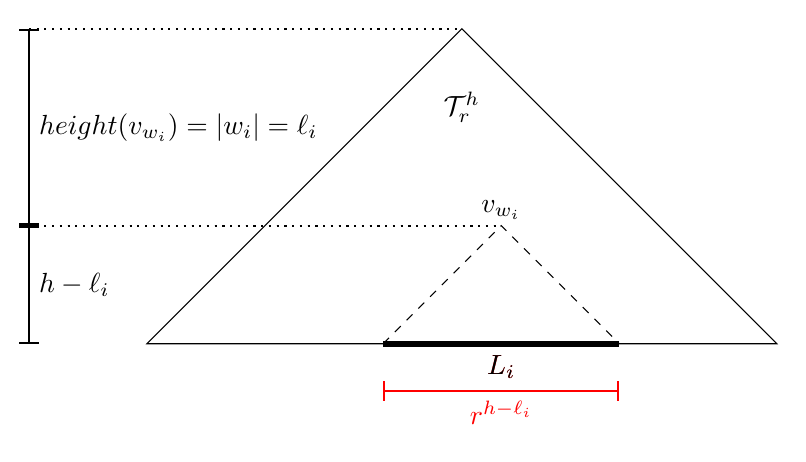
\begin{tikzpicture}
            \node at (0,-1) {$\mathcal{T}_r^h$};
            \node at (.5, -2.3) {$v_{w_i}$};

            \draw (0,0)
                -- (-4,-4)
                -- (4,-4)
                -- cycle;

            \draw[dashed] (-1,-4) -- (.5, -2.5) -- (2,-4);

            \only<1>{
                \draw[line width = 2pt,red] (-1,-4) -- (2,-4);
                \node[color=red] at (.5, -4.3) {$L_i$};
            }

            \visible<2->{
                \node at (.5, -4.3) {$L_i$};
                \draw[line width = 2pt] (-1,-4) -- (2,-4);
                \draw[dotted, line width = .8pt] (-5.5, -2.5) -- (.5, -2.5);

                \draw[dotted, line width = .8pt] (-5.5, 0) -- (0, 0);
                \draw[|-|, line width = .8pt] (-5.5,-2.5) --
                    node[right] {$height(v_{w_i}) = |w_i| = \ell_i$} (-5.5, 0);
                \draw[dotted, line width = .8pt] (-5.5, -2.5) -- (.5, -2.5);
                \draw[|-|, line width = .8pt] (-5.5,-4) -- node[right] {$h-\ell_i$} (-5.5, -2.5);
                \draw[|-|, line width = .8pt,color=red] (-1,-4.6) -- node[below] {$r^{h-\ell_i}$} (2,-4.6);
            }
        \end{tikzpicture}

    \end{center}
\end{frame}

\begin{frame}[t]
    \frametitle{Ungleichung von Kraft: ''$\,\Longleftarrow\,$''}
    \begin{itemize}
        \setlength\itemsep{1em}
        \item $L_i \cap L_j = \varnothing$ für $i \neq j$.
        \item $|L_i| = r^{h-\ell_i}$
    \end{itemize}\strut\\[10pt]

    $$
        r^h \ \geq\ \left| \bigcup_{i \in [1,q]} L_i \right|
    \visible<2->{
        \ =\ \sum_{i=1}^{q} |L_i|
        \ =\ \sum_{i=1}^{q} r^{h-\ell_i}
        \ =\ r^h\sum_{i=1}^{q} \frac{1}{r^{\ell_i}}
    }
    $$
    \visible<3->{
    $$
        \,\Longleftrightarrow\, \sum_{i=1}^{q} \frac{1}{r^{\ell_i}} \leq 1
    $$
    \strut\hfill$\square$
    }
\end{frame}

\begin{frame}[t]
    \frametitle{Ungleichung von Kraft}
    Seien $q,r \in \mathbb{N}, \ell \in \mathbb{N}^q$. Dann existiert ein $r$-ärer sofort dekodierbarer Code $\mathcal{C}$
    mit Wortlängen $\ell$ genau dann, wenn
    $$
        \sum_{k=1}^{q} \frac{1}{r^{\ell_k}} \leq 1
    $$
    \begin{itemize}
        \setlength\itemsep{1em}
        \item Beweis konstruktiv
        \item Untere Schranke für Wortlänge, Alphabetgröße
        \setlength\itemsep{3em}
        \pause
        \item Bekannt: sofort dekodierbar $\,\Longrightarrow\,$ eindeutig dekodierbar
        \setlength\itemsep{1em}
        \item Schwächere Kriterien?
    \end{itemize}
\end{frame}

\begin{frame}[t]
    \frametitle{Ungleichung von McMillan}
    Seien $q,r \in \mathbb{N}, \ell \in \mathbb{N}^q$.
    Dann existiert ein $r$-ärer {\color{red}eindeutig dekodierbarer} Code $\mathcal{C}$
    mit Wortlängen $\ell$ genau dann, wenn
    \begin{equation}
        K := \sum_{k=1}^{q} \frac{1}{r^{\ell_k}} \leq 1
    \end{equation}\\[20pt]

    Richtung ''$(1) \,\Longrightarrow\, \mathcal{C}$ existiert'' durch Kraft.\\
\end{frame}

\begin{frame}[t]
    \frametitle{Ungleichung von McMillan: Beweisidee}
    \begin{itemize}
        \setlength\itemsep{1.3em}
        \item Zu zeigen: $K = \sum_{k=1}^{q} \frac{1}{r^{\ell_k}} \leq 1$
        \item Betrachte $K^n$ abhängig von Wortlängen für beliebiges $n \in \mathbb{N}$.
        \item Finde aus Form von $K^n$ konstante obere Schranke
        \item Dann muss $K \leq 1$, da sonst $K^n$ für geeignetes $n$ größer
            als jede Konstante
    \end{itemize}
\end{frame}

\begin{frame}[t]
    \frametitle{Ungleichung von McMillan: ''$\,\Longleftarrow\,$''}
        Zu zeigen: $K \leq 1$, wobei
        $\displaystyle
            K = \sum_{k=1}^{q} \frac{1}{r^{\ell_k}}
        $.\\
        \pause
        Für $n \in \mathbb{N}$ ist:
        $$
            K^n = \left(\sum_{k=1}^{q} \frac{1}{r^{\ell_k}}\right)^n
            \pause
            = \sum_{i \in [1,q]^n} \prod_{k=1}^{n} \frac{1}{r^{\ell_{i_k}}}
            \pause
            = \sum_{i\in [1,q]^n} r^{-\sum_{k=1}^{n} \ell_{i_k}}
        $$\pause
        Dann für jedes $i \in [1,q]^n:$
        $$
            n\cdot \ell_{min} \leq \sum_{k=1}^{n} \ell_{i_k} \leq n\cdot \ell_{max}
        $$
        \pause
        Wir wollen schreiben:
        $$
            K^n
            \ =\ \sum_{i\in [1,q]^n} r^{-\sum_{k=1}^{n} \ell_{i_k}}
            \ =\ \sum_{j=n\cdot \ell_{min}}^{n\cdot \ell_{max}} {\color{red}N_j}\cdot r^{-j}
        $$
\end{frame}

\begin{frame}[t]
    \frametitle{Ungleichung von McMillan: ''$\,\Longleftarrow\,$''}
    Ziel: Gleiche Summenwerte durch ${\color{red}N_j} \in \mathbb{N}_0$ zusammenfassen
    $$
        K^n = \sum_{i\in [1,q]^n} r^{-\sum_{k=1}^{n} \ell_{i_k}}
        = \sum_{j=n\cdot\ell_{min}}^{n\cdot\ell_{max}} {\color{red}N_j} \cdot r^{-j}
    $$
    \pause

    \begin{itemize}
        \setlength\itemsep{1em}
        \item $N_j$ Anzahl $i \in [1,q]^n$ mit Wortlängensumme $j$
        \pause
        \item Äquivalent: Anzahl $i \in [1,q]^n$ mit $|w_{i_1}w_{i_2}\dots w_{i_n}| = j$
        \pause
        \item $\mathcal{C}$ eindeutig dekodierbar
            $\,\Longrightarrow\,$ Jede Code-Sequenz aus eindeutiger Auswahl
                $i \in [1,q]^n$
        \pause
    \item $r^j$ Wörter mit Länge $j$, nicht alles Code-Sequenzen von $\mathcal{C}$
    \item Für jedes max. ein $i \in [1,q]^n \,\Longrightarrow\, N_j \leq r^j$
    \end{itemize}

\end{frame}

\begin{frame}[t]
    \frametitle{Ungleichung von McMillan: ''$\,\Longleftarrow\,$''}
        Mit {\only<2>{\color{red}}$N_j \leq r^j$} folgt:
        $$
            K^n
            \ =\ \sum_{j = n\cdot \ell_{min}}^{n\cdot \ell_{max}} N_jr^{-j}
            \ =\ \sum_{j = n\cdot\ell_{min}}^{n\cdot\ell_{max}} \frac{N_j}{r^j}
        $$
        \pause
        $$
            \quad{\color{red}\leq}\quad \sum_{j = n\cdot\ell_{min}}^{n\cdot\ell_{max}} 1
            \quad=\quad n(\ell_{max}-\ell_{min}) + 1
        $$
        \pause
        \strut
        $$
            \,\Longrightarrow\, \frac{K^n}{n}\ \leq\ (\ell_{max}-\ell_{min}) + 1
        $$
\end{frame}

\begin{frame}[t]
    \frametitle{Ungleichung von McMillan: ''$\,\Longleftarrow\,$''}
        $$
            \frac{K^n}{n}\ \leq\ (\ell_{max}-\ell_{min}) + 1
        $$
        \begin{itemize}
            \setlength\itemsep{1em}
            \item Code $\mathcal{C}$ gegeben: $q,r,\ell$ fix.
            \item Damit auch $\ell_{min},\ell_{max}, K$ fix.
            \pause
            \item $n \in \mathbb{N}$ beliebig; Ungleichung muss für alle $n \in \mathbb{N}$ gelten.
            \item Nach Analysis/DSAL bekannt: nur möglich für $K \leq 1$.
        \end{itemize}
        \strut\\
        $$
            \,\Longrightarrow\, \sum_{i=1}^{q} \frac{1}{r^{\ell_i}} = K \leq 1
        $$
        \strut\hfill$\square$
\end{frame}

\begin{frame}[t]
    \frametitle{Bemerkungen}
    Für $r,q \in \mathbb{N}, \ell \in \mathbb{N}^q$ ergibt sich:
    $$
        \exists \mathcal{C}_{r,q,\ell}\ \text{eindeutig dekodierbar}
        \quad\Longleftrightarrow\quad
        \exists \mathcal{C}'_{r,q,\ell}\ \text{sofort dekodierbar}
    $$
    \pause
    Außerdem, für festen Code $\mathcal{C}_{r,q,\ell}:$
    $$
        \sum_{i=1}^{q} \frac{1}{r^{\ell_i}} \leq 1
        \quad\xcancel{\large\ \Longrightarrow\ }\quad
        \mathcal{C}_{r,q,\ell}\ \text{sofort dekodierbar}
    $$
    \pause
    Beispiel: $r=2,q=3,\ell=(1,2,3)$
    $$
        \sum_{i=1}^{q} \frac{1}{r^{\ell_i}}
        \ =\ \frac{1}{2^1} + \frac{1}{2^2} + \frac{1}{2^3}
        \ =\ \frac{7}{8}
        \ <\ 1
    $$
    $$
        \mathcal{C} := \{0,01,011\}\ \text{\textbf{nicht} sofort dekodierbar!}
    $$
\end{frame}


\begin{frame}[t]
    \frametitle{Zusammenfassung}

    \begin{itemize}
        \setlength\itemsep{1em}
        \item Existenz der Codes abhängig von:\\
            Alphabetgröße($r$), Anzahl Codewörter($q$), Codewortlängen($\ell$)
        \item Genauer durch Ungleichung von Kraft/McMillan:
            $$
                \sum_{i=1}^{q} \frac{1}{r^{\ell_i}} \leq 1
            $$
        \item Zusammenhang/Konstruktion von Codes durch Bäume
    \end{itemize}

\end{frame}

\end{document}
